\section{Installation} % Dar más detalles
In order to use \ThesiX{} clone or download the whole repository at https://github.com/ilomdez/ThesiX. Compiling the code should be pretty straight forward, although some steps might vary depending on the operative system and the compiler chosen:

\subsection{Windows - TextMaker - MikTex}
This section has been tested under Windows 10, TexMaker 5.0.3 and MikTex 2.9.6972. The version of each package used in the compilation of the latest \ThesiX{} manual can be found in the log file in the main folder of the repository.

Follow the instructions below:
\begin{enumerate}
	\item Download the corresponding MikTex version (https://miktex.org/download) and install it.
	\item Download the corresponding TexMaker version (https://www.xm1math.net/texmaker/) and install it.
	\item Configure TexMaker as depicted in \fig\,\ref{fig:Intro_TexMakerConf}.
	\item If you want to make use of the commands to allow the use of svg images
	\item If you want to make use of the commands to allow the use of tif images

\end{enumerate}

%%%%%%%%%%%%%%%%%%
\begin{figure}[h]
    \centering
    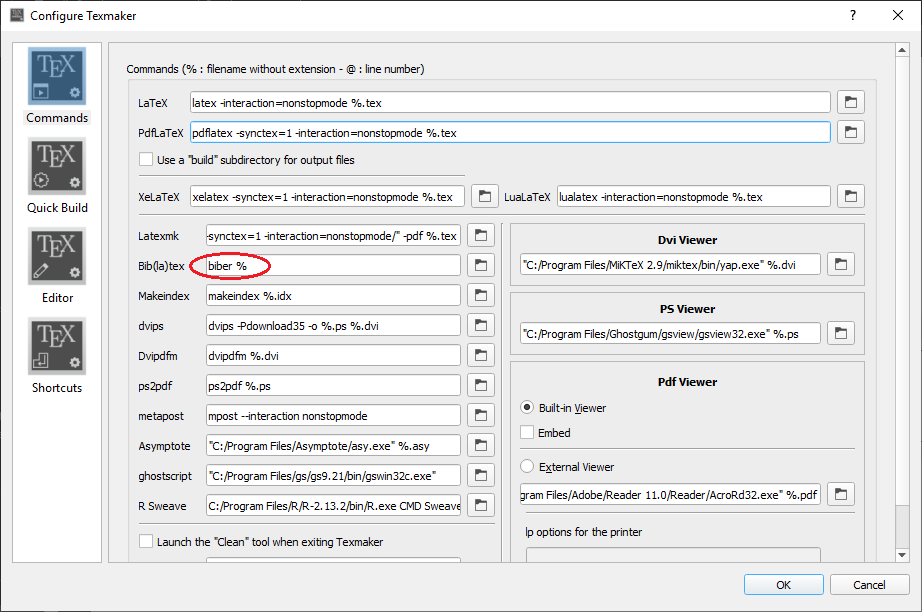
\includegraphics[width=.95\textwidth]{Intro_TexMakerConf.png}
    \caption[Screenshot of the main configuration settings in TexMaker.]{Screenshot of the main configuration settings in TexMaker.}
    \label{fig:Intro_TexMakerConf}    
\end{figure}
%%%%%%%%%%%%%%%%%%

\subsection{Windows - TexStudio - MikTex}
Coming soon!

\subsection{Linux}
Coming soon!
